%%%%%%%%%%%%%%%%% DO NOT CHANGE HERE %%%%%%%%%%%%%%%%%%%% 
%%%%%%%%%%%%%%%%%%%%%%%%%%%%%%%%%%%%%%%%%%%%%%%%%%%%%%%%%%{
    \documentclass[twoside,11pt]{article}
    %%%%% PACKAGES %%%%%%
    \usepackage{pgm2016}
    \usepackage{amsmath}
    \usepackage{algorithm}
    \usepackage[noend]{algpseudocode}
    \usepackage{subcaption}
    \usepackage[english]{babel}	
    \usepackage{paralist}	
    \usepackage[lowtilde]{url}
    \usepackage{fixltx2e}
    \usepackage{listings}
    \usepackage{color}
    \usepackage{hyperref}
    \usepackage{geometry}

    \geometry{a4paper,scale=0.8}
    \usepackage{auto-pst-pdf}
    \usepackage{pst-all}
    \usepackage{pstricks-add}
    
  
    %arabic 阿拉伯数字
    %roman 小写的罗马数字
    %Roman 大写的罗马数字
    %alph 小写字母
    %Alph 大写字母
    %%%%% MACROS %%%%%%
    \algrenewcommand\Return{\State \algorithmicreturn{} }
    \algnewcommand{\LineComment}[1]{\State \(\triangleright\) #1}
    \renewcommand{\thesubfigure}{\roman{subfigure}}
    \definecolor{codegreen}{rgb}{0,0.6,0}
    \definecolor{codegray}{rgb}{0.5,0.5,0.5}
    \definecolor{codepurple}{rgb}{0.58,0,0.82}
    \definecolor{backcolour}{rgb}{0.95,0.95,0.92}
    \lstdefinestyle{mystyle}{
       backgroundcolor=\color{backcolour},  
       commentstyle=\color{codegreen},
       keywordstyle=\color{magenta},
       numberstyle=\tiny\color{codegray},
       stringstyle=\color{codepurple},
       basicstyle=\footnotesize,
       breakatwhitespace=false,        
       breaklines=true,                
       captionpos=b,                    
       keepspaces=true,                
       numbers=left,                    
       numbersep=5pt,                  
       showspaces=false,                
       showstringspaces=false,
       showtabs=false,                  
       tabsize=2
    }
    \lstset{style=mystyle}
%%%%%%%%%%%%%%%%%%%%%%%%%%%%%%%%%%%%%%%%%%%%%%%%%%%%%%%%%% 
%%%%%%%%%%%%%%%%%%%%%%%%%%%%%%%%%%%%%%%%%%%%%%%%%%%%%%%%%% }

%%%%%%%%%%%%%%%%%%%%%%%% CHANGE HERE %%%%%%%%%%%%%%%%%%%% 
%%%%%%%%%%%%%%%%%%%%%%%%%%%%%%%%%%%%%%%%%%%%%%%%%%%%%%%%%% {
\newcommand\course{SCEE08010}
\newcommand\courseName{Engineering Math 2B}
\newcommand\semester{Winter 2020}
\newcommand\assignmentNumber{1}                             % <-- ASSIGNMENT #
\newcommand\studentName{Jiaqing Xie}                  % <-- YOUR NAME
\newcommand\studentEmail{J.Xie-21@sms.ed.ac.uk}          % <-- YOUR NAME
\newcommand\studentNumber{s2001696}                % <-- STUDENT ID #
%%%%%%%%%%%%%%%%%%%%%%%%%%%%%%%%%%%%%%%%%%%%%%%%%%%%%%%%%% }
%%%%%%%%%%%%%%%%%%%%%%%%%%%%%%%%%%%%%%%%%%%%%%%%%%%%%%%%%%

%%%%%%%%%%%%%%%%% DO NOT CHANGE HERE %%%%%%%%%%%%%%%%%%%% 
%%%%%%%%%%%%%%%%%%%%%%%%%%%%%%%%%%%%%%%%%%%%%%%%%%%%%%%%%%
%{

    \ShortHeadings{University of Edinburgh -  \course ~~ \courseName}{\studentName - \studentNumber}
    \firstpageno{1}
    
    \begin{document}
    
    \title{Probability \& Statistics Coursework}
    
    \author{\name \studentName \email \studentEmail \\
    \studentNumber
    \addr
    }
    
    \maketitle
%%%%%%%%%%%%%%%%%%%%%%%%%%%%%%%%%%%%%%%%%%%%%%%%%%%%%%%%%%
%%%%%%%%%%%%%%%%%%%%%%%%%%%%%%%%%%%%%%%%%%%%%%%%%%%%%%%%%% }



The solution of the coursework is shown below. R code can be found in the last part of this document. According to the latex code and more information about the Brownian motion and stochastic process, it can be found at my Github repository: \url{https://github.com/JIAQING-XIE/Engineering-Mathematics-2B}


 \renewcommand\thesection{\alph{section}}
\section{Recursive Calculation}
\label{sec:background}

%%EXAMPLE EQUATION

The formula given in the question a) has been shown in (1) and (4). We can easily achieve the following series of equations with the number of j.


\begin{align}
    X_{1} &= x_{0} + \upsilon\delta t + \sigma W_{1}\sqrt{\delta t}\\
    X_{2} &= X_{1} + \upsilon\delta t + \sigma W_{2}\sqrt{\delta t}\\
    \cdots\\
    X_{j} &= X_{j-1} + \upsilon\delta t + \sigma W_{j}\sqrt{\delta t}
\end{align}
It's convenient to add the terms of the left side of the equations, as well as the right side of the equations listed above separately, abridging to only one equation in (5).
\begin{align}
\sum_{i=1}^{j}X_{i} &= \sum_{i=1}^{j-1}X_{i} + x_{0} +j\upsilon\delta t+\sigma \sum_{i=1}^{j}W_{i}\sqrt{\delta t}
\end{align}
It can be soon simplified to:
\begin{align}
X_{j} =  x_{0} +j\upsilon\delta t+\sigma \sum_{i=1}^{j}W_{i}\sqrt{\delta t}
\end{align}
Therefore, it doesn't depend on the previous position. Instead, it's a function of $W_{i}$(i = 1, 2, ..., j) and the parameters($x_{0}$, $\upsilon$, $\sigma$, $\delta$t and j).
%EXAMPLE MULTIPLE TABLES TABLE


\section{Mean, Variance and Covariance}

The information has been given that $W_{i}$(i = 1, 2, ... ,j) are independent standard normal random variables. We can set another variable $Y_{j}$ which is equal to $\sum_{i=1}^{j}W_{i}$.

\begin{equation}
\left\{
             \begin{array}{lr}
             W_{i} \sim N(0,1) \\
              & 1\leq i\leq j\\
             Y_{j}=\sum_{i=1}^{j}W_{i} \sim N(0,j)
             \end{array}
\right.
\end{equation}

Now we rewrite the equation(6) to equation(8):
\begin{align}
    X_{j} =  x_{0} +j\upsilon\delta t+\sigma\sqrt{\delta t}Y_{j}
\end{align}
Then we can get the distribution of $X_{j}$: 
\begin{align}
    X_{j} \sim N(x_{0} +j\upsilon\delta t, j\sigma^{2}\delta t)\\
    E(X_{j}) = x_{0} +j\upsilon\delta t\\
    Var(X_{j}) = j\sigma^{2}\delta t
\end{align}
$X_{j}$ is normally distributed. The mean and variance are $x_{0} +j\upsilon\delta t$ and  j$\sigma^{2}\delta t$ respectively.

\begin{equation}
    \begin{split}
        E(X_{j}X_{k}) &= E((x_{0} +j\upsilon\delta t+\sigma\sqrt{\delta t}Y_{j})(x_{0} +k\upsilon\delta t+\sigma\sqrt{\delta t}Y_{k}))\\
        &= E((x_{0}+ j\upsilon\delta t)(x_{0} +k\upsilon\delta t) + (x_{0} +k\upsilon\delta t)\sigma\sqrt{\delta t}Y_{j} +(x_{0} +j\upsilon\delta t)\sigma\sqrt{\delta t}Y_{k} + \sigma^{2}\delta tY_{j}Y_{k})\\
        &= E((x_{0}+ j\upsilon\delta t)(x_{0} +k\upsilon\delta t)) + E((x_{0} +k\upsilon\delta t)\sigma\sqrt{\delta t}Y_{j})+E((x_{0} +j\upsilon\delta t)\sigma\sqrt{\delta t}Y_{k}) +E(\sigma^{2}\delta tY_{j}Y_{k})
    \end{split}
\end{equation}
Conditions are:
\begin{equation}
\left\{
             \begin{array}{lr}
             E((x_{0} +k\upsilon\delta t)\sigma\sqrt{\delta t}Y_{j}) = 0 \\
             E((x_{0} +j\upsilon\delta t)\sigma\sqrt{\delta t}Y_{k}) =0\\
             E(\sigma^{2}\delta tY_{j}Y_{k}) = \sigma^{2}\delta tE(\sum_{i=1}^{k}\sum_{m=1}^{k}W_{i}W_{m})\\
             \end{array}
\right.
\end{equation}
Since $W_{i}$ are independent variables,  E($W_{j}W_{k}$ )= E($W_{j}$)E($W_{k}$)=0 if j $\neq$ k.
\begin{equation}
    \sigma^{2}\delta tE(\sum_{i=1}^{j}\sum_{m=1}^{k}W_{i}W_{m}) = 
            \begin{array}{lr}
                \sigma^{2}\delta t\sum_{i=1}^{j}E(W_{i}^{2}) &j<k\\
                \sigma^{2}\delta t\sum_{i=1}^{k}E(W_{i}^{2}) &k<j\\
             \end{array}
\end{equation}
\begin{equation}
    \begin{split}
    E(W_{i}^{2}) &= Var(W_{i}) + (E(W_{i}))^{2}\\
    &= 1 + 0\\
    &= 1
    \end{split}
\end{equation}
Therefore, equation (14) can be rewritten to:
\begin{equation}
    \sigma^{2}\delta tE(\sum_{i=1}^{j}\sum_{m=1}^{k}X_{i}X_{m}) = 
            \begin{array}{lr}
                j\sigma^{2}\delta t &j<k\\
                k\sigma^{2}\delta t &k<j\\
             \end{array}\\
    = min\{j,k\}*\sigma^{2}\delta t
\end{equation}
Therefore, 
\begin{equation}
    \begin{split}
        Cov(X_{j}, X_{k}) &= E(X_{j}X_{k})-E(X_{j})E(X_{k})\\
        &= E((x_{0}+ j\upsilon\delta t)(x_{0} +k\upsilon\delta t)) + min\{k,j\}\sigma^{2}\delta t - E(x_{0} + j\upsilon\delta t)E(x_{0} + k\upsilon\delta t)\\
        &=  min\{k,j\}*\sigma^{2}\delta t \neq 0 
    \end{split}
\end{equation}
So $X_{j}$ and $X_{k}$ are not independent.

\section{Joint Normal}
\begin{align}
    X_{i} \sim N(x0 + i\upsilon\delta t, i\sigma^{2}\delta t)\\
    a_{i}X_{i} \sim N(a_{i}(x0 + i\upsilon\delta t), a_{i}^{2}(i\sigma^{2}\delta t))
\end{align}
We treat the term $a_{i}X_{i}$ as the new variable $Z_{i}$ which serves normal distribution. \\
Property: If X $\sim$ N($\mu_{1}$, $\sigma_{1}^{2}$), Y $\sim$ N($\mu_{2}$, $\sigma_{2}^{2}$),then Z = mX + nY $\sim$ N($m\mu_{1}+n\mu_{2}$, $m^{2}\sigma_{1}^{2}+n^{2}\sigma_{2}^{2}$).Therefore,
\begin{align}
    \sum_{i=1}^{n}Z_{i} \sim N(\sum_{i=1}^{n}a_{i}(x0 + i\upsilon\delta t),\sum_{i=1}^{n}a_{i}^{2}(i\sigma^{2}\delta t))
\end{align}
Therefore, it serves the normal distribution, which means that $X_{1}, X_{2},...,X_{n}$ are jointly normal.


\section{Joint Density}
Considering the case for n=3:
\begin{equation}
    \begin{split}
    \sum_{ij} = Cov\{X_{i}, X_{j}\} &= 
    min\{i,j\}*\sigma^{2}\delta t\\
    &= \sigma^{2}\delta t
\left (
\begin{matrix}
1 & 1 & 1 \\
1 & 2 & 2 \\
1 & 2 & 3
\end{matrix}
\right )
    \end{split}
\end{equation}
The inverse of the matrix(21) is equal to:
\begin{align}
    \frac{1}{\sigma^{2}\delta t}
    \left (
\begin{matrix}
2 & -1 & 0 \\
-1 & 2 & -1 \\
0 & -1 & 1 
\end{matrix}
\right )
\end{align}
We have x $\in$ $R^{3}$. Therefore, x = $(x_{1}, x_{2},x_{3})^{T}$, $\mu$ = $(\mu_{1}, \mu_{2}, \mu_{3})^{T}$. The  exponential term inside equals to:


\begin{equation}
    \begin{split}
    &= \frac{1}{2\sigma^{2}\delta t}
    \left (
\begin{matrix}
x_{1}-\mu_{1} & x_{2}-\mu_{2}  &x_{3}-\mu_{3}\\
\end{matrix}
\right )
\left (
\begin{matrix}
2 & -1 & 0 \\
-1 & 2 & -1 \\
0 & -1 & 1 
\end{matrix}
\right )
 \left (
\begin{matrix}
x_{1}-\mu_{1} \\
x_{2}-\mu_{2}\\
x_{n}-\mu_{3}
\end{matrix}
\right )\\
&= \frac{1}{2\sigma^{2}\delta t}
\left (
\begin{matrix}
2(x_{1}-\mu_{1})-(x_{2}-\mu_{2})
&-(x_{1}-\mu_{1})+2(x_{2}-\mu_{2})-(x_{3}-\mu_{3})  &-(x_{2}-\mu_{2})+(x_{3}-\mu_{3})\\
\end{matrix}
\right )
\left (
\begin{matrix}
x_{1}-\mu_{1} \\
x_{2}-\mu_{2}\\
x_{3}-\mu_{3}
\end{matrix}
\right )\\
&= \frac{1}{2\sigma^{2}\delta t}[(x_{1}-\mu_{1})^{2} + ((x_{2}-\mu_{2})-(x_{1}-\mu_{1}))^{2} + ((x_{3}-\mu_{3})-(x_{2}-\mu_{2}))^{2}]\\
&= \frac{1}{2\sigma^{2}\delta t}[(x_{1}-x_{0}-\upsilon\delta t)^{2} + (x_{2}-x_{1}-\upsilon\delta t)^{2} +(x_{3}-x_{2}-\upsilon\delta t)^{2}]
    \end{split}
\end{equation}
Replace the following formula (24) with formula (23).

\begin{equation}
    \begin{split}
    p(x) &= \frac{1}{{2\pi}^{\frac{n}{2}}}|det{\sum}^{-1}|^{\frac{1}{2}}exp(-\frac{1}{2}(x-\mu)^{T}{\sum}^{-1}(x-\mu))\\
    &= \frac{1}{{2\pi}^{\frac{3}{2}}}(\frac{1}{\sigma^{2}\delta t})^{\frac{3}{2}}exp(-\frac{1}{2\sigma^{2}\delta t}[(x_{1}-x_{0}-\upsilon\delta t)^{2} + (x_{2}-x_{1}-\upsilon\delta t)^{2} +(x_{3}-x_{2}-\upsilon\delta t)^{2}])\\
    &= \frac{1}{\sqrt{2\pi}}\frac{1}{\sqrt{\sigma^{2}\delta t}}e^{-\frac{(x_{1}-x_{0}-\upsilon\delta t)^{2}}{2\sigma^{2}\delta t}} * \frac{1}{\sqrt{2\pi}}\frac{1}{\sqrt{\sigma^{2}\delta t}}e^{-\frac{(x_{2}-x_{1}-\upsilon\delta t)^{2}}{2\sigma^{2}\delta t}} *\frac{1}{\sqrt{2\pi}}\frac{1}{\sqrt{\sigma^{2}\delta t}}e^{-\frac{(x_{3}-x_{2}-\upsilon\delta t)^{2}}{2\sigma^{2}\delta t}}\\
    &= \prod_{j=1}^{3}\frac{1}{\sqrt{2\pi}\sqrt{\sigma^{2}\delta t}}exp(-\frac{(x_{j}-x_{j-1}-\upsilon\delta t)^{2}}{2\sigma^{2}\delta t})
    \end{split}
\end{equation}
And we have the assumption that when x$\in$ $R^{n}$ p(x) can be written to:

\begin{align}
    p(x) = \prod_{j=1}^{n}\frac{1}{\sqrt{2\pi}\sqrt{\sigma^{2}\delta t}}exp(-\frac{(x_{j}-x_{j-1}-\upsilon\delta t)^{2}}{2\sigma^{2}\delta t})
\end{align}

\section{Independence and Physical Explanation}

To prove that the random variables $X_{1}, X_{2}, ..., X_{j-1}$ are independent of $X_{j}, ..., X_{n}$ given $X_{j} = x \in R$, it is equivalent to prove that p($X_{1}, ..., X_{j-1}|X_{j} = x$)p($X_{j+1}, ..., X_{n}|X_{j} = x$) = p($X_{1},...,X_{j-1},X_{j+1},...,X_{n}|X_{j} = x$).
Observing the equation (1) that is given in question d, $p(x_{j})$ is equivalent to $p(x_{j} = x|x_{j-1})$ in this case. It has no connection with $x_{j-2},...,x_{1}$. It's a great example of Markov process. So from the given equation (1) we have:
\begin{align}
    p(x_{1},...,x_{j-1},x_{j}) &= p(x_{1})\prod_{i=2}^{j}p(x_{i}|x_{i-1})\\
    p(x{j},x_{j+1},x_{j+2},...,x_{n}) &= \prod_{i=j}^{n}p(x_{i}|x_{i-1})
\end{align}
\begin{equation}
    \begin{split}
        p(x_{1},...,x_{j-1}|x_{j} = x) &= \frac{p(x_{1},...,x_{j-1},x_{j} = x)}{p(x_{j} = x|x_{j-1})}\\
        &= \frac{p(x_{1})\prod_{i=2}^{j}p(x_{i}|x_{i-1})}{p(x_{j} = x|x_{j-1})}\\
        p(x_{j+1},...,x_{n}|x_{j } = x) &= \frac{p(x_{j} = x,x_{j+1},...,x_{n})}{p(x_{j} = x|x_{j-1})}\\
        &= \frac{\prod_{i=j}^{n}p(x_{i}|x_{i-1})}{p(x_{j} = x|x_{j-1})}\\
        p(x_{1},...,x_{j-1}|x_{j} = x)p(x_{j+1},...,x_{n}|x_{j} = x) &= \frac{p(x_{1})\prod_{i=2}^{n}p(x_{i}  |x_{i-1})p(x_{j} = x|x_{j-1})}{p(x_{j} = x|x_{j-1})p(x_{j} = x|x_{j-1})}\\
        &= \frac{p(x_{1},...,x_{n})}{p(x_{j} = x|x_{j-1})}\\
        &= p(x_{1},...,x_{j-1},x_{j+1},...,x_{n}|x_{j} = x)
    \end{split}
\end{equation}
It satisfies the equation p($X_{1}, ..., X_{j-1}|X_{j} = x$)p($X_{j+1}, ..., X_{n}|X_{j} = x$) = p($X_{1},...,X_{j-1},X_{j+1},...,X_{n}|X_{j}$).So variables $X_{1}, X_{2}, ..., X_{j-1}$ are independent of $X_{j+1}, ..., X_{n}$.
The physical explanation for this independence is that the article doesn't record the previous coordinate that it has moved to. Also, it doesn't affect the future movement of the article. The next movement only depends on the current state. Totally, it's a memoryless system, which is a specific stochastic process.

\section{Maximum Likelihood Estimation}
The answer is to calculate MLE($\hat{x_{0}}, \hat{\sigma},\hat{\upsilon}$). It needs to calculate $\hat{x_{0}}, \hat{\sigma}$ and $\hat{\upsilon}$ separately.
According to the value of the function, L(${x_{0}}, {\sigma},{\upsilon}$;x) is equal to p(x;${x_{0}}, {\sigma},{\upsilon}$). But they have different meanings in the probability domain(L($\theta$;x) is the posterior probability distribution while p(x;$\theta$) is the probability distribution function. However we can ignore their conceptual difference here, because the aim is to make the estimation.
\begin{equation}
    \left\{
             \begin{array}{lr}
              \hat{x_{0}} &= \underset{x_{0}}{\operatorname{argmin}}(-log(L({x_{0}};x)))\\
             \hat{\sigma} &= \underset{\sigma}{\operatorname{argmin}}(-log(L({\sigma};x)))\\
             \hat{\upsilon} &= \underset{\upsilon}{\operatorname{argmin}}(-log(L({\upsilon};x)))\\
             
             \end{array}
\right.
\end{equation}
We can simplify the log term:
\begin{equation}
    \begin{split}
       log(L({x_{0}}, {\sigma},{\upsilon};x)) &= log( \prod_{j=1}^{n}\frac{1}{\sqrt{2\pi}\sqrt{\sigma^{2}\delta t}}exp(-\frac{(x_{j}-x_{j-1}-\upsilon\delta t)^{2}}{2\sigma^{2}\delta t}))  \\
       &= -nlog(\sqrt{2\pi}\sqrt{\sigma^{2}\delta t}-\sum_{j=1}^{n}\frac{(x_{j}-x_{j-1}-\upsilon\delta t)^{2}}{2\sigma^{2}\delta t}
    \end{split}
\end{equation}
From equation (30), we can infer that:
\begin{align}
    \frac{\partial({-log(L({x_{0}};x}))}{\partial{x_{0}}} =0 \\
    \frac{\partial({nlog(\sqrt{2\pi}\sqrt{\sigma^{2}\delta t}+\sum_{j=1}^{n}\frac{(x_{j}-x_{j-1}-\upsilon\delta t)^{2}}{2\sigma^{2}\delta t}})}{\partial{x_{0}}} =0\\
    \frac{x_{1}-x_{0}-\upsilon\delta t}{\sigma^{2}\delta t} =0\\
    \hat{x_{0}} = x_{1} - \upsilon\delta t
    \Longrightarrow \hat{x_{0}} = x_{0} + \sigma W_{1}\sqrt{\delta t}
\end{align}
From equation (30), we can infer that:
\begin{align}
    \frac{\partial({-log(L({\upsilon;x}))}}{\partial{\upsilon}} =0 \\
    \frac{\partial({nlog(\sqrt{2\pi}\sqrt{\sigma^{2}\delta t}+\sum_{j=1}^{n}\frac{(x_{j}-x_{j-1}-\upsilon\delta t)^{2}}{2\sigma^{2}\delta t}})}{\partial{\upsilon}} =0\\
    \sum_{j=1}^{n}\frac{2\delta t(x_{j}-x_{j-1}-\upsilon\delta t )}{2\sigma^{2}\delta t} =0\\
    n\delta t \upsilon = \sum_{j=1}^{n}x_{j}-x_{j-1}\\
    n\delta t \hat{\upsilon} = n\upsilon\delta t+\sigma \sum_{i=1}^{n}W_{i}\sqrt{\delta t}
    \Longrightarrow \hat{\upsilon} = \upsilon +\frac{\sigma \sum_{i=1}^{n}W_{i}}{n\sqrt{\delta t}}
\end{align}
From equation (30), we can infer that:
\begin{align}
    \frac{\partial({-log(L({\sigma};x}))}{\partial{\sigma}} =0 \\
    \frac{\partial({nlog(\sqrt{2\pi}\sqrt{\sigma^{2}\delta t}+\sum_{j=1}^{n}\frac{(x_{j}-x_{j-1}-\upsilon\delta t)^{2}}{2\sigma^{2}\delta t}})}{\partial{\sigma}} =0\\
    \frac{n}{\sigma} -\frac{\sum_{j=1}^{n}(x_{j}-x_{j-1}-\upsilon\delta t)^{2}}{\sigma^{3}\delta t} =0\\
    \hat{\sigma} = \sqrt{\frac{\sum_{j=1}^{n}(x_{j}-x_{j-1}-\upsilon\delta t)^{2}}{n\delta t}}
    \Longrightarrow \hat{\sigma} =\sigma \sqrt{\frac{\sum_{j=1}^{n}W_{j}^{2}}{n}}
\end{align}
Therefore, the maximum likelihood estimation for the drift $\upsilon$ is equal to $\upsilon +\frac{\sigma \sum_{i=1}^{n}W_{i}}{n\sqrt{\delta t}}$. MLE for the initial location $x_{0}$ is equal to $ x_{0} + \sigma W_{1}\sqrt{\delta t}$. MLE for the diffusion term $\sigma$ is equal to $\sigma \sqrt{\frac{\sum_{j=1}^{n}W_{j}^{2}}{n}}$

\section{Simulation of Brownian Motion in R}

%% EXAMPLE ALGORITHM
\begin{lstlisting}[language=R]
vx <- 0.5; #parameter setting
vy <- 0.2; 
delta_t <- 0.0001;
sigma <- 1;
xdis <- sigma*sqrt(delta_t)*rnorm(99, 0 ,1) + delta_t*vx ; # x coordinate
ydis <- sigma*sqrt(delta_t)*rnorm(99, 0 ,1) + delta_t*vy ; # y coordinate
xdis = cumsum(xdis);# sum the value in the array before i.
ydis = cumsum(ydis);
xdims <- append(xdis,c(0),after=0); # make sure that the start point is (0,0)
ydims <- append(ydis,c(0),after=0);
plot(xdims, ydims, type="l", main =" Brownian Motion in Two Dimension", xlab="x coordinate", ylab = "y coordinate"); # make a 2-dimensional plot.
\end{lstlisting}
\begin{figure}[ht]
    \centering
    \begin{minipage}[t]{0.45\textwidth}
    \centering
        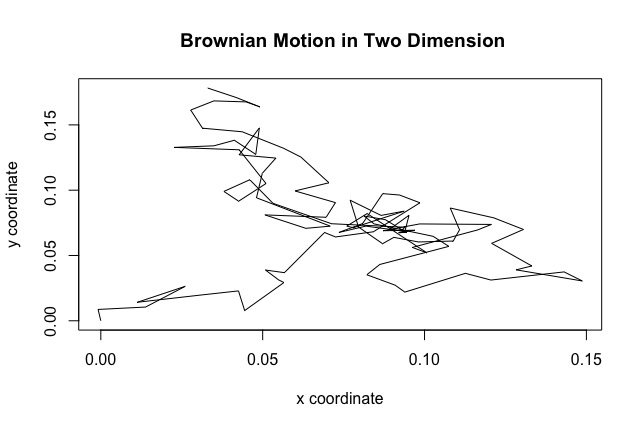
\includegraphics[width=7.7cm]{Brownian Motion(1).jpeg}
        \caption{Simulation1,N=100}
    \end{minipage}
    \begin{minipage}[t]{0.46\textwidth}
    \centering
        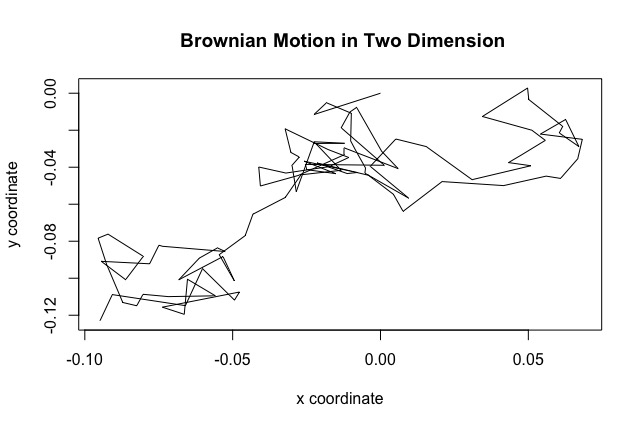
\includegraphics[width=7.7cm]{Brownian Motion(2).jpeg}
        \caption{Simulation2,N=100}
    \end{minipage}
    \centering
    \begin{minipage}[t]{0.45\textwidth}
    \centering
        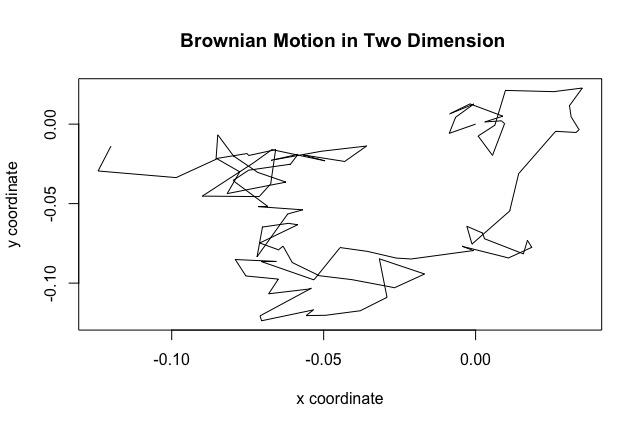
\includegraphics[width=7.7cm]{Brownian Motion(3).jpeg}
        \caption{Simulation3,N=100}
    \end{minipage}
    \begin{minipage}[t]{0.46\textwidth}
    \centering
        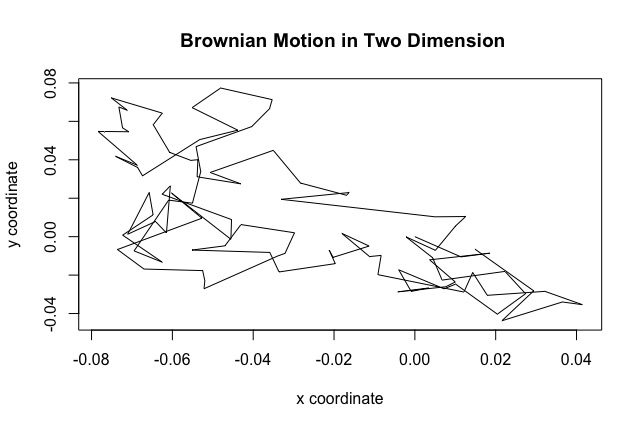
\includegraphics[width=7.7cm]{Brownian Motion(4).jpeg}
        \caption{Simulation4,N=100}
    \end{minipage}
    \begin{minipage}[t]{0.46\textwidth}
    \centering
        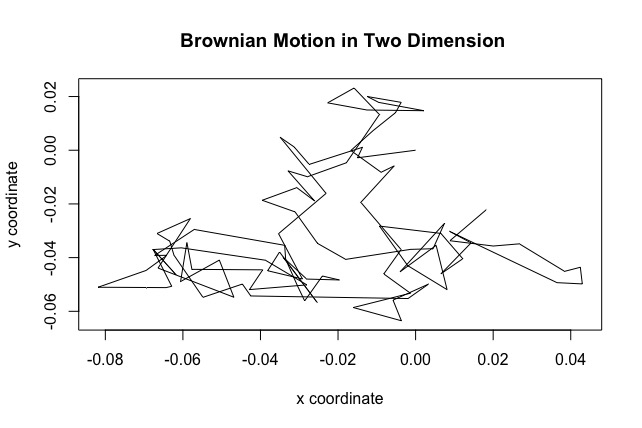
\includegraphics[width=7.0cm]{Brownian Motion(5).jpeg}
        \caption{Simulation5,N=100}
    \end{minipage}
\end{figure}   
The code is shown in the page 6, which is used to simulate the path of the particle in a short time increment with 100 paths. Plots are also implemented with the plot function in R.

I have done more experiments on the simulation of Brownian Motion by changing not only path numbers but also the dimensions, which present more tricky but also interesting images.
\begin{figure}[ht]
    \centering
    \begin{minipage}[t]{0.45\textwidth}
    \centering
        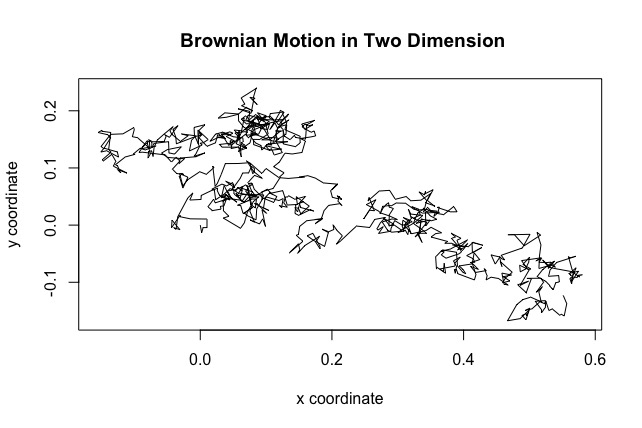
\includegraphics[width=7.7cm]{Brownian Motion(6).jpeg}
        \caption{Simulation6,N=1000}
    \end{minipage}
    \begin{minipage}[t]{0.46\textwidth}
    \centering
        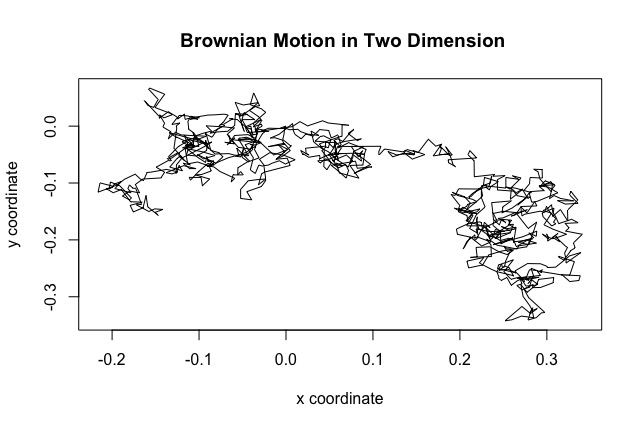
\includegraphics[width=7.7cm]{Brownian Motion(7).jpeg}
        \caption{Simulation7,N=1000}
    \end{minipage}
    \centering
    \begin{minipage}[t]{0.45\textwidth}
    \centering
        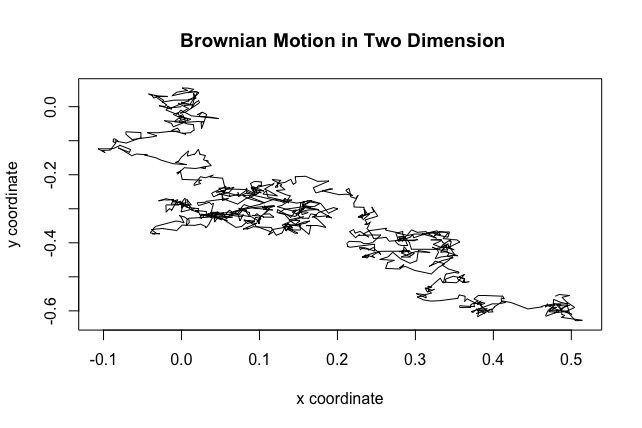
\includegraphics[width=7.7cm]{Brownian Motion(8).jpeg}
        \caption{Simulation8,N=1000}
    \end{minipage}
    \begin{minipage}[t]{0.46\textwidth}
    \centering
        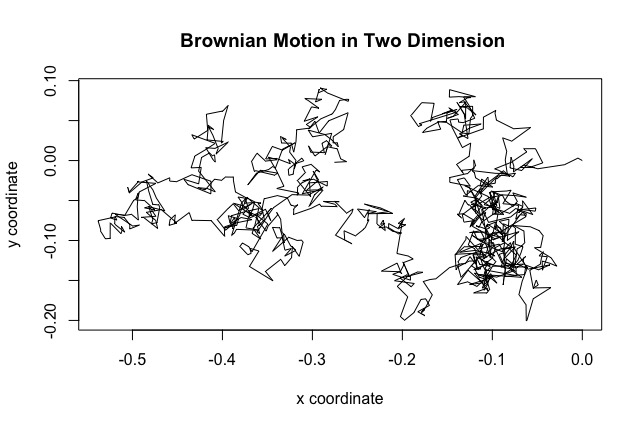
\includegraphics[width=7.7cm]{Brownian Motion(9).jpeg}
        \caption{Simulation9,N=1000}
    \end{minipage}
    \begin{minipage}[t]{0.46\textwidth}
    \centering
        \includegraphics[width=7.7cm]{3d(1).jpeg}
        \caption{3D-Simulation1,N=5000}
    \end{minipage}
    \begin{minipage}[t]{0.46\textwidth}
    \centering
        \includegraphics[width=7.7cm]{3d(2).jpeg}
        \caption{3D-Simulation2,N=5000}
    \end{minipage}
\end{figure}   












\end{document}
